\documentclass[11pt,a4paper]{article}


\setlength{\topmargin}{-55pt}%
\setlength{\oddsidemargin}{-20pt}%
\setlength{\textwidth}{490pt}%
\setlength{\textheight}{700pt}%
\setlength{\headsep}{20pt}%
\setlength{\headheight}{14pt}

\usepackage[utf8]{inputenc} % accents 8 bits dans le fichier
\usepackage[T1]{fontenc}      % accents codés dans la fonte
\usepackage[french]{babel}
\usepackage{amsmath,amssymb}
\usepackage{graphicx}
\usepackage{fancyhdr}
\usepackage{booktabs}
\usepackage{color, colortbl}
\usepackage{appendix}
\usepackage{pgfplots}
\usepackage[hidelinks]{hyperref}
\usepackage{siunitx}
\usepackage{algorithmicx}
\usepackage{algorithm}
\usepackage{algpseudocode}
\usepackage{subcaption}

\pgfplotsset{compat=1.3}

\addto\captionsfrench{% Replace "english" with the language you use
  \renewcommand{\contentsname}%
    {Table des matières}
}

\DecimalMathComma

\lhead{}      %en-tête
\chead{MPNA : Méthode des itérations simultanées}%
\rhead{}%
\lfoot{\tiny{Pierre GRANGER \& Matthias BEAUPERE}}
\cfoot{}%
\rfoot{\thepage}%
\renewcommand{\headrulewidth}{0.5pt}
\renewcommand{\footrulewidth}{0.5pt}
\pagestyle{fancy}

\newcommand{\HRule}{\rule{\linewidth}{0.5mm}}
\newcommand{\norm}[1]{\left\lVert#1\right\rVert}

\definecolor{green}{rgb}{0.2,0.8,0.2}

\begin{document}
\begin{center}

	{\LARGE\centering Projet de MPNA :\\ Méthode des itérations simultanées}\\[1cm]

	{ Matthias \bsc{Beaupère}, Pierre \bsc{Granger}}\\[0.5cm]
	{Rapport MPNA - CHPS - \today}\\[2cm]
\end{center}

\tableofcontents
\newpage

\section{Introduction et position du problème}
	De nombreux problèmes modernes impliquent le calcul de valeurs propres et de vecteurs propres de grandes matrices creuses. Par exemple, ce problème peut être rencontré lors de l'étude de certains systèmes physiques ou bien par exemple dans les moteurs de recherche qui reposent sur ce type de technique. Des algorithmes spécifiques doivent être utilisés afin de résoudre ces problèmes de valeur propre en un temps raisonnable. De plus les algorithmes utilisés doivent pouvoir être facilement utilisés sur les architectures massivement parallèles actuelles ce qui représente un grand défi.

\section{Approche utilisée}

\section{Cas séquentiel}

	\subsection{Description de l'algorithme général}

		Données du problèmes :

		\begin{itemize}
			\item $M$ : taille du sous-espace de Krylov
			\item $k$ : nombre de vecteurs propres demandé
			\item $p$ : précision demandé
			\item $A$ : matrice de taille $n*n$ donnée en entrée
			\item $N_{iter}$ : nombre d'itérations
		\end{itemize}
		\vspace{1cm}
		L'algorithme \ref{alg:global} détail l'implémentation globale de la méthode des itérations simultanées.

		\begin{algorithm}
			\caption{Algorithme général}
			\label{alg:global}
			\begin{algorithmic}[1]
					\State $Q \gets rand()$
					\While {$i = 0 .. N_{iter}-1$ OU max(precisions) < p}
						\State $Z = AQ$
						\State Gram-Schmidt $Q$
						\State Projection $B = Z^tAZ$
						\State Décomposition de Schur $B = Y^tRY$
						\State Retour dans l'espace d'origine $Q = ZY$
						\State Calcul de la précision des vecteurs de $Q$
						\State Sélection des $k$ vecteur propres
					\EndWhile
				\end{algorithmic}
		\end{algorithm}

		Dans les paragraphes suivant sont détaillés chaque étape de l'algorithme.

		\subsubsection{Procédé de Gram-Schmidt}

		On utilise une décomposition QR avec le procédé de Gram-Schmidt pour orthonormalisé la matrice Q. L'ortogonalisation consiste à ajouter chaque vecteur de la matrice $Z$ dans une vecteur temporaire tout en lui soustrayant son projeté sur chaque vecteur déjà ajouté. On normalise ensuite en divisant chaque vecteur par sa norme. L'implémentation est présenté dans l'algorithme \ref{alg:gm}.

			\begin{algorithm}
				\begin{algorithmic}[1]
					\For {$i = 0..m-1$}
						\State $q^{temp}_i \gets q_i$
						\For{$k = 0..i$}
						\State $q^{temp}_i \gets q^{temp}_i - q_k(q_k.q_i)$
						\EndFor
					\EndFor
					\For {$i = 0..m-1$}
						\State $q_i \gets \frac{q_i^{temp}}{\norm{q_i^{temp}}}$
					\EndFor
				\end{algorithmic}
				\caption{Algorithme de Gram-Schmidt}
				\label{alg:gm}
			\end{algorithm}

		\subsubsection{Décomposition de Schur}

		La décomposition de Schur permet de calculer les valeurs et vecteurs propre de l'espace de Krylov, aussi appelés valeurs et vecteurs de Ritz. Pour ce calcul a été utilisé la bibliothèque \texttt{lapacke}.

		\subsubsection{Calcul de la précision}

			Pour calculer la précision de chaque vecteur propre, on compare le vecteur propre avec son produit par la matrice $A$ donnée en entrée. On donne ci-dessous la formule pour le vecteur propre i.

			$$
			p_i = \norm{Aq-\lambda q}
			$$

		\subsubsection{Sélection de $k$ vecteurs propres}

			En entrée du programme est précisé le nombre $k$ de vecteurs propres désirés. La précision est calculé uniquement sur les $k$ vecteurs de plus grande valeur propre associée. On suppose que les vecteurs de plus grande valeur propre associée sont ceux qui ont la meilleure précision. On sélectionne donc les $k$ vecteurs de $Q$ qui ont la plus grande précision.

	\subsection{Étude de performances théorique}
		
		\subsubsection{Objectif en précision ou en itération}
			
			La terminaison du programme est donnée par deux critères suivant les paramètres entrée par l'utilisateur :
			\begin{itemize}
				\item Un objectif en précision : pour un exposant $p$ donné en argument, le programme termine si les $k$ vecteurs propres ont une précision inférieure à $10^{-p}$.
				\item Un objectif en itération : pour un entier $i$ donné en entrée, le programme termine si on atteint l'itération $i$.
			\end{itemize}

			Pour les formules de complexité, on supposera que l'objectif est de $N_{iter}$ itérations, même si en pratique le calcul s'arrête dans le cas où l'objectif en précision est spécifié et atteint avant l'objectif en itération.

		\subsubsection{Calcul de complexité}

			Exprimons la complexité totale de l'algorithme des itérations simultanées sous le forme de la somme des complexités des opérations qui le composent.

			$$
			\fbox{$C^{tot} = N_{iter} (C^{AQ} + C^{GM} + C^{Proj} + C^{Schur} + C^{mm} + C^{preci} + C^{select})$}
			$$

			Détaillons maintenant chaque terme de cette somme.

			\paragraph{Produit $AQ$ :} On effectue le produit de $A \in \mathbb{R}^{N\times N}$ par $Q \in \mathbb{R}^{N \times M}$. On a donc la complexité
			$$C^{AQ} = O(N^2M)$$

			\paragraph{Procédé de Gram-Schmidt :} L'algorithme de Gram-Schmidt se décompose en deux étape indépendantes :
			\begin{itemize}
				\item l'othogonalisation consiste à un produit scalaire entre de vecteur de taille N dans une double boucle couvrant l'intervalle $\{(i,j) | i \in [0,M-1] et j \in [O,i]\}$. Le cardinal de cet intervalle est $(M)log(M)$, ce qui donne une complexité $O(NMlog(M))$ pour l'orthogonalisation
				\item la normalisation consiste en $M-1$ produits scalaires de vecteurs de taille N, ce qui donne une complexité $O(NM)$ pour la normalisation.
			\end{itemize}		
			La complexité pour le procédé de Gram-Schmidt est donc
			
			$$C^{GM} = O(NMlog(M))$$

			\paragraph{Projection :} Il s'agit d'un produit entre la matrice $Z^t \in \mathbb{R}^{M\times N}$ et la matrice $A \in \mathbb{R}^{N\times N}$ puis un produit entre la matrice résultante et la matrice $Z$. Ces produits matriciels on tous les deux la complexité $O(MN^2)$. Ce qui donne une complexité pour l'étape de projection
			
			$$C^{Proj} = C^{mm} = O(N^2M)$$

			\paragraph{Décomposition de Schur :} La décomposition de Schur est effectué sur l'espace de taille $M \times N$. Comme on a $N \gg M$ on peut négliger la complexité introduit par cette étape du calcul. Donc

			$$C^{Schur} \approx 0$$

			\paragraph{Précision :} La précision se calcule pour les $M$ vecteurs de la matrice $Q$. Pour chaque vecteur on calcule $\norm{Aq-\lambda q}$.
			\begin{itemize}
				\item Le produit $Aq$ se calcule avec un complexité $O(NM)$
				\item Le produit $\lambda q$ se calcule avec une complexité $O(N)$
				\item La norme se calcule avec une complexité $O(N)$
			\end{itemize}
			
			Ce qui donne une complexité totale de
			$$C^{preci} = O(NM^2)$$

			\paragraph{Sélection :} La sélection des k vecteurs propres de plus grande précision est de l'ordre de grandeur de $M$, ce qui est négligeable devant les autres complexités qui dépendent de $N$.
			
			$$C^{select} \approx 0$$


		\subsubsection{Complexité totale}
			
			D'après les calculs de chaque complexité, on la complexité totale suivanté :

			$$
			C^{tot} = N_{iter}(O(N^2M) + O(NMlog(M)) + O(N^2M) + O(NM^2))
			$$
			
			Le terme dominant de la somme est $O(N^2M)$ relatif à la projection et au produit $AQ$. On obtient donc après avoir négligé les autres termes la complexité

			$$ 
			\fbox{$C^{tot} = O(N_{iter}N^2M)$}
			$$




	\subsection{Étude de performances pratique}



	\subsection{Ajout d'une méthode de déflation "Locking"}
		Toutes les valeurs propres de la matrice possèdent une vitesse de convergence différente par la méthode des itérations simultanées. Cela nous amène à affiner et recalculer constamment des vecteurs déjà connus avec la bonne précision ce qui entraine une perte de temps de calcul. De plus, des vecteurs propres qui ont déjà convergés jusqu'à la bonne précision peuvent perdre en précision à cause d'instabilités numériques au fil des calculs : la précision de certains vecteurs propres peut osciler au cours des itérations.

		Afin de résoudre ces deux problèmes nous avons décidé de mettre en place une méthode de déflation appelée "locking". Le principe est simple : lorsqu'un vecteur propre a convergé jusqu'à la précision désirée, on le verrouille de sorte à ne plus le remultiplier par la matrice $A$ et on diminue la taille du sous-espace de Krylov d'une unité. Néanmoins, on utilise toujours ce vecteur pour l'orthonormalisation afin qu'il guide la convergence correcte des veteurs restants.

	\subsection{Conclusions}

\section{Cas parallèle}
	\subsection{Approche utilisée}
		Maintenant que nous avons correctement pu tester notre code séquentiel et valider les résultats que nous obtenons avec, nous nous attachons à paralléliser notre implémentation. Tout d'abord, il faut remarquer que nous effectuons des calculs dans deux espaces vectoriels différents : dans l'espace d'origine $\mathbb{R}^{N\times N}$ et dans le sous-espace de Krylov $\mathbb{R}^{m\times m}$. Les calculs les plus couteux sont donc bien évidemment ceux effectués dans l'espace d'origine qui est une dimension largement supérieure à celle du sous-espace de Krylov. Les calculs qu'il est donc nécessaire de paralléliser sont ceux effectués dans l'espace d'origine ainsi que les changements de base pour passer de l'espace d'origine au sous-espace de Krylov. Les calculs à paralléliser sont donc les produits matrice/matrice dans l'espace d'origine.

		Afin de paralléliser les produits matriciels, on commence par l'implémentation la plus simple et la plus efficace qui consiste à effectuer une parallélisation en mémoire partagée grâce à OpenMP car la plupart des calculs sont indépedants lors du produit matriciel et que l'on peut gérer efficacement les réductions. De plus, puisque la mémoire est partagée, il n'y a pas de pénalités en temps de communication.

	\subsection{Étude de performances théorique}
	\subsection{Étude de performances pratique}
	\subsection{Conclusions}

\section{Conclusion générale}

	Nous avons pu implémenter la méthode des itérations simultanées afin de calculer les valeurs et vecteurs propres d'une grande matrice creuse. Nous avons ensuite tenté d'améliorer l'algorithme initialement proposé en introduisant le "locking" permettant de modifier les paramètres de redémarrage afin de gagner à la fois en temps de calcul et en stabilité numérique de la convergence. Nous avons pu constater que l'ajout du locking a effectivement permis d'augmenter l'efficacité et la précision de notre implémentation. Nous avons aussi implémenté un conditionnement simpliste des matrices en entrée afin de résoudre certains problèmes de stabilité numérique dans le cas de matrices mal conditionnées en entrée.

	Nous nous sommes ensuite proposés de paralléliser notre programme à l'aide de deux outils : OpenMP et MPI. Nous avons tout d'abord effectué la parallélisation des boucles avec OpenMP puis nous avons implémenté les produits de matrices couteux en MPI. Nous avons pu tester notre code parallèle sur le cluster poincare à la maison de la simulation. Les résultats furent assez décevants car notre parallélisation MPI a augmenté les temps de calcul à cause des coups trop élevés des transferts de données. Nous en concluons que la parallélisation efficace de ce type d'algoithme doit plutôt reposer sur l'implémentation de méthodes hybrides.


% FIGURES A AJOUTER
\begin{figure}
	\centering
	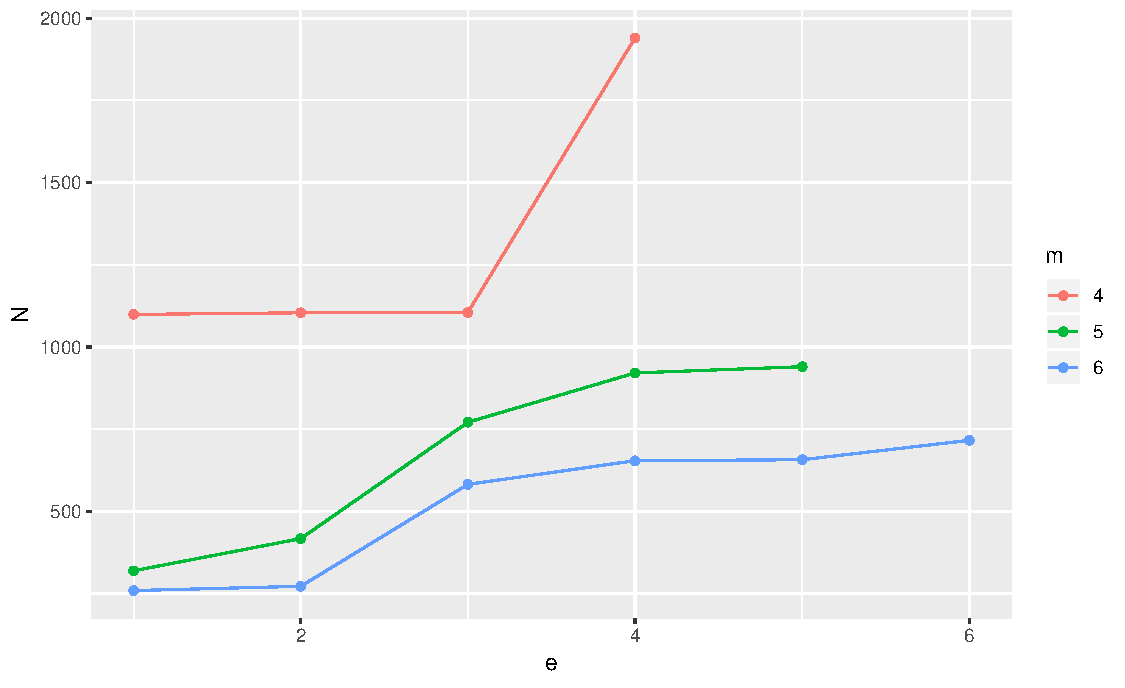
\includegraphics[width=0.8\linewidth, keepaspectratio]{plots/Nvse-m_p6.pdf}
	\caption{Nombre d'itérations $N$ nécessaires pour faire converger $e$ valeurs propres pour différentes tailles de sous-espace de Krylov $m$ et une précision $p=\SI{e-6}{}$ \label{fig:Nvse-m_p6}}
\end{figure}

\begin{figure}
	\centering
	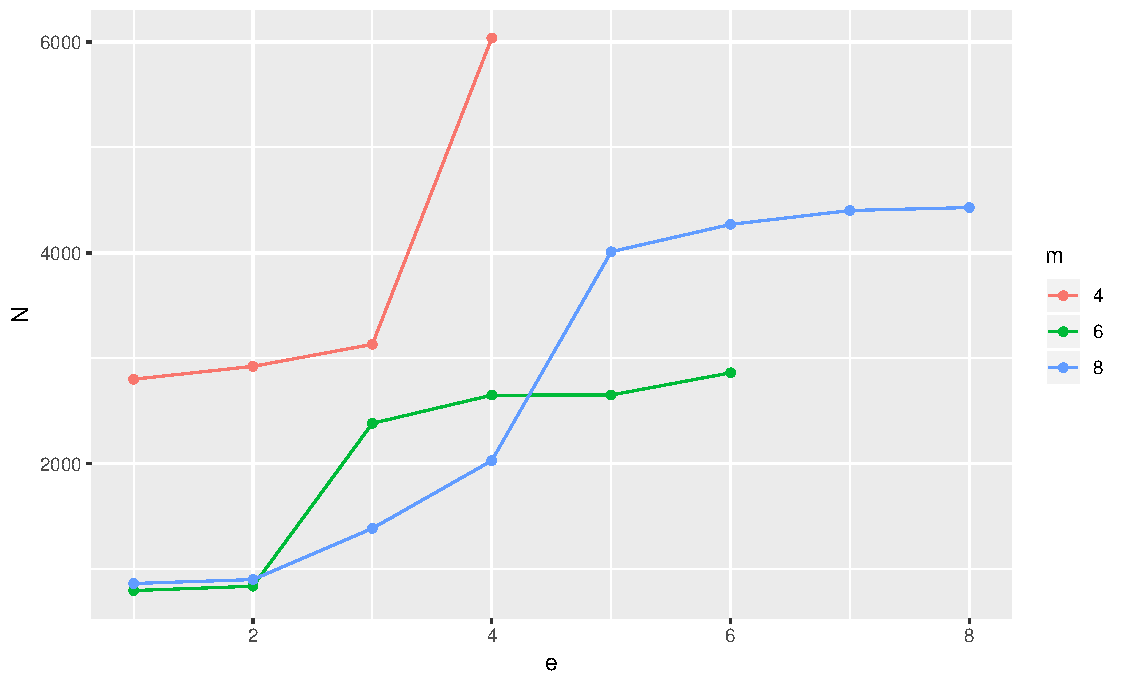
\includegraphics[width=0.8\linewidth, keepaspectratio]{plots/Nvse-m_p8.pdf}
	\caption{Nombre d'itérations $N$ nécessaires pour faire converger $e$ valeurs propres pour différentes tailles de sous-espace de Krylov $m$ et une précision $p=\SI{e-8}{}$ \label{fig:Nvse-m_p8}}
\end{figure}

\begin{figure}
	\centering
	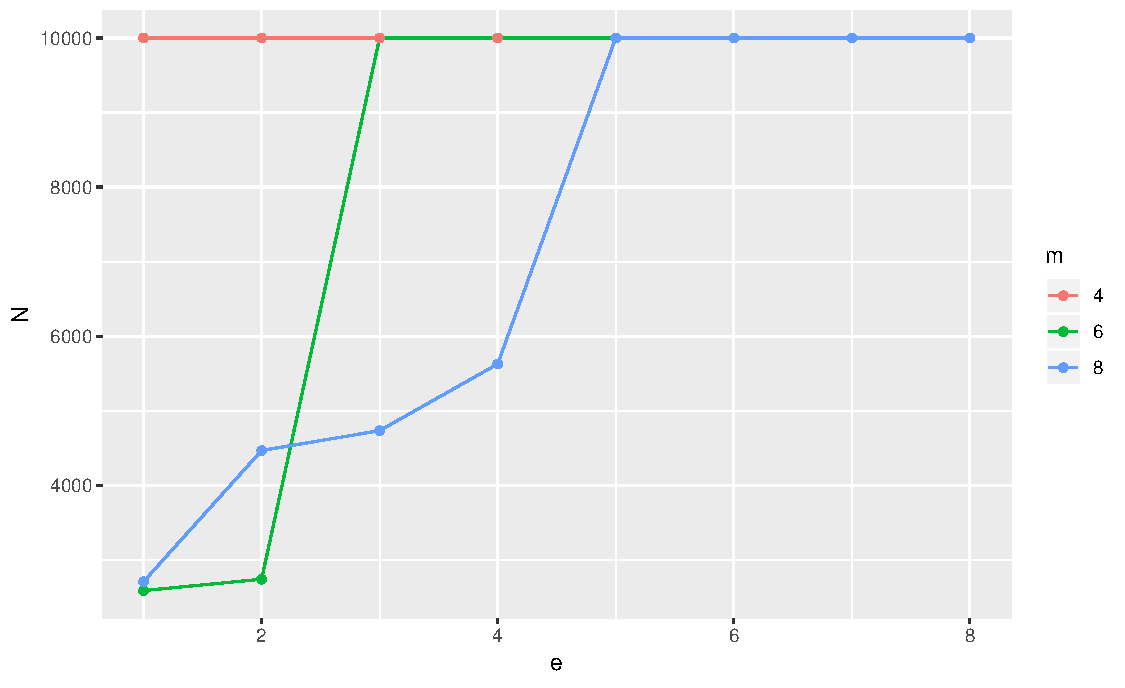
\includegraphics[width=0.8\linewidth, keepaspectratio]{plots/Nvse-m_p10.pdf}
	\caption{Nombre d'itérations $N$ nécessaires pour faire converger $e$ valeurs propres pour différentes tailles de sous-espace de Krylov $m$ et une précision $p=\SI{e-10}{}$ \label{fig:Nvse-m_p10}}
\end{figure}

\begin{figure}
	\centering
	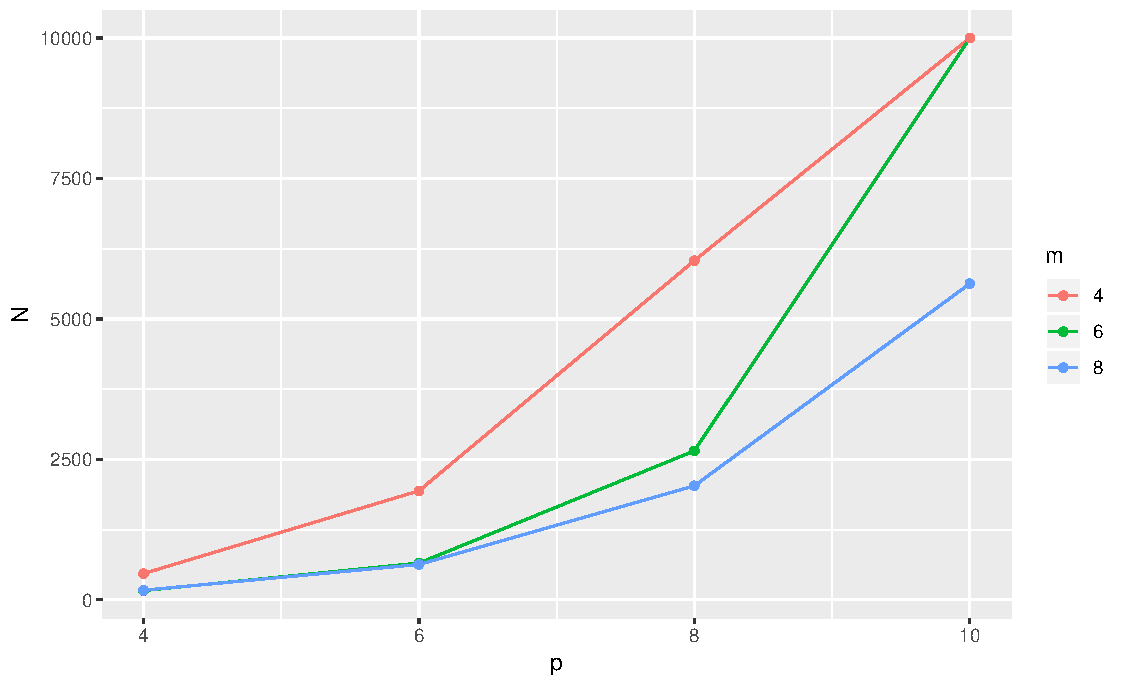
\includegraphics[width=0.8\linewidth, keepaspectratio]{plots/Nvsp-m_e4.pdf}
	\caption{Nombre d'itérations $N$ nécessaires pour faire converger $e = 4$ valeurs propres pour différentes tailles de sous-espace de Krylov $m$ et une précision $p$ \label{fig:Nvsp-m_e4}}
\end{figure}

\begin{figure}
	\centering
	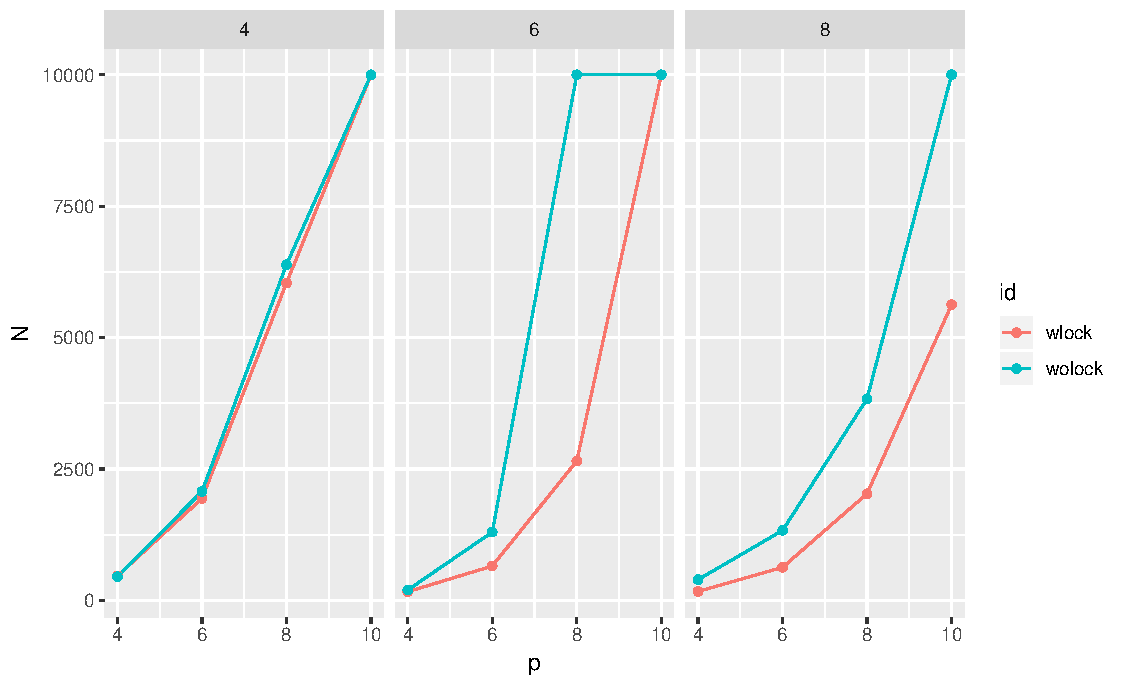
\includegraphics[width=0.8\linewidth, keepaspectratio]{plots/Nvsp_complock.pdf}
	\caption{Nombre d'itérations $N$ nécessaires pour faire converger $e = 4$ valeurs propres pour différentes tailles de sous-espace de Krylov $m$ et une précision $p$ avec et sans utilisation du locking \label{fig:Nvsp_complock}}
\end{figure}

\begin{figure}
	\centering
	\begin{subfigure}{0.49\linewidth}
		\centering
		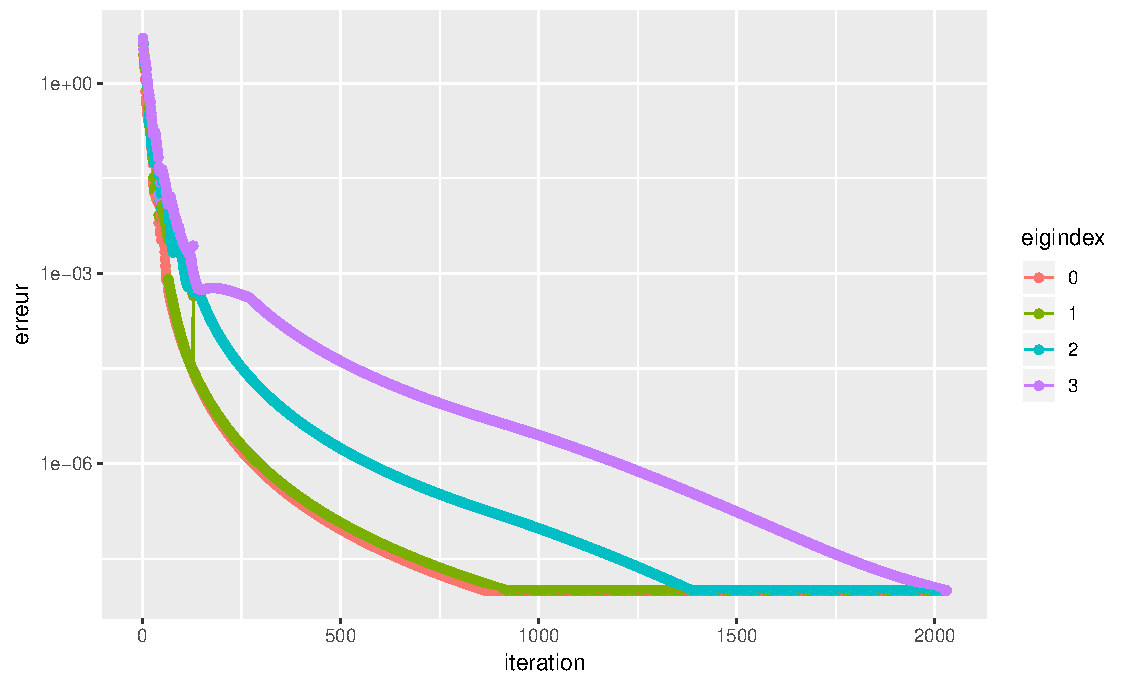
\includegraphics[width=\linewidth, keepaspectratio]{plots/wlock_e4_p8_m8.pdf}
		\caption{Avec locking\label{wlock_e4_p8_m8}}
	\end{subfigure}
	\begin{subfigure}{0.49\linewidth}
		\centering
		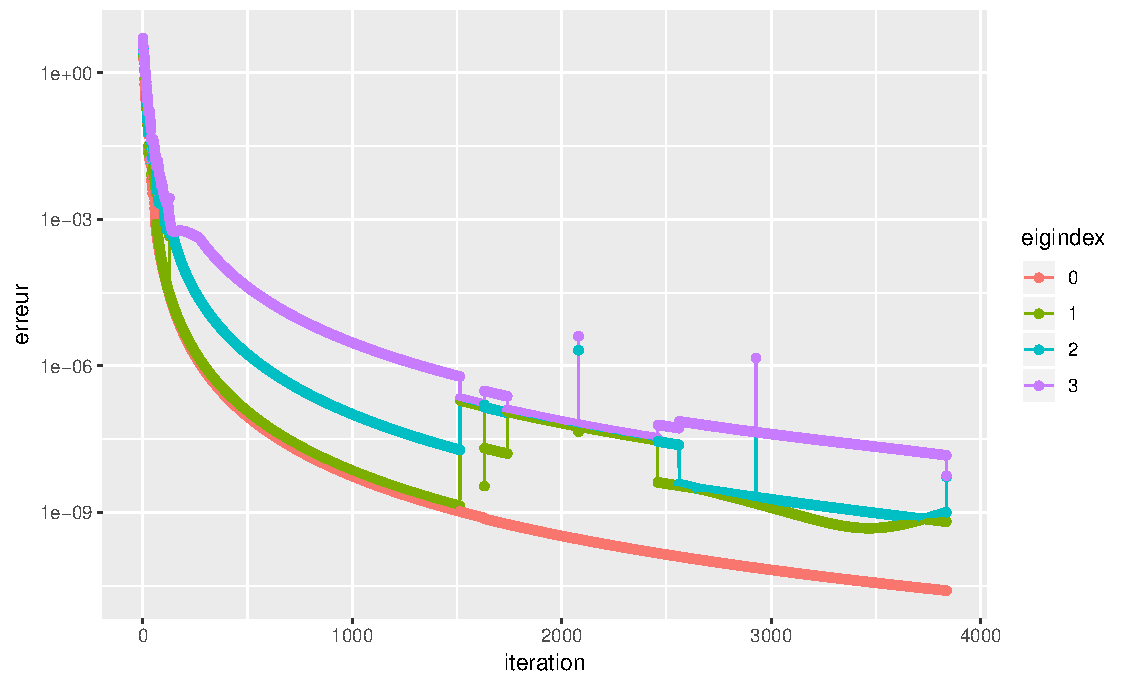
\includegraphics[width=\linewidth, keepaspectratio]{plots/wolock_e4_p8_m8.pdf}
		\caption{Sans locking\label{wolock_e4_p8_m8}}
	\end{subfigure}
	\caption{Précision au cours des itérations $N$ pour $e = 4$ valeurs propres pour une taille de sous-espace de Krylov $m=8$\label{fig:comp_locks}}
\end{figure}

On représente sur la figure \ref{fig:comp_locks} la précision au cours des itérations pour $e$ et $m$ fixés dans le cas de la méthode initiale et de la méthode avec locking. On peut tout d'abord observer que la convergence est bien plus rapide lorsque le locking est utilisé (environ 2000 contre 3800 itérations). On peut en outre constater sur la figure \ref{wlock_e4_p8_m8} que la convergence avec locking semble moins instable.


% \bibliographystyle{unsrt}
% \bibliography{synopsis.bib}

%\input{appendix}

\end{document}
